\section{Asymmetry-Aware Links}
\label{sec:interconnect}

Figure~\ref{fig:symmetric_assymetric}(a) shows a generic multi-socket system
with symmetric bandwidth assignments at each inter-socket communication link.
Each link is comprising multiple equal number of uni-directional high-speed
lanes in both directions collectively comprising a symmetric bi-directional
link.  Static link capacity assignment at design time is very common and has
multiple advantages. For example, in such case only one type of I/O circuitry
(egress drivers or ingress receivers) along with only one type of control logic
need to be implemented at each on-chip link interface. Moreover, multi-socket
switches result in simpler designs that support a statically provisioned
bandwidth scenario. On the other hand, multi-socket link bandwidth has a very
important impact on overall system performance. For the applications which
saturate links between sockets, doubling NVLink capacity potentially achieves a
2$\times$ speedup. As I/O bandwidth is a very limited and expensive resource,
this result motivates us to look for alternatives that keep wire and I/O
resources at very high utilization. 

We make a new observation that the typically employed symmetric link capacity
assignments may result in lower overall utilization of the link wires in many
cases. Moreover, in case of multi-socket NUMA GPU systems, we do observe that
there are applications in which some GPUs have a very different utilization of
its egress and ingress channels in different phases of execution.
Figure~\ref{fig:link-motivation} shows dynamic link utilization for a snapshot
of \texttt{HPC-HPGMG-UVM} application running on our baseline 4 GPUs
multi-scocket system. Vertical dotted black lines represent the beginning
kernel calls that are split across 4 sockets as explained in
Section~\ref{sec:background}. We can see that few initial small kernels have a
negligible interconnect utilization on all links. However, for the upcoming
larger kernels at the figure, GPU0 and GPU2 fully saturate their ingress links,
while GPU1 and GPU3 fully saturate their egress links. At the same time GPU0 
and GPU2 pair, and GPU1 and GPU3 pair barely use their egress or ingress links.

\begin{figure}[t]
    \centering
    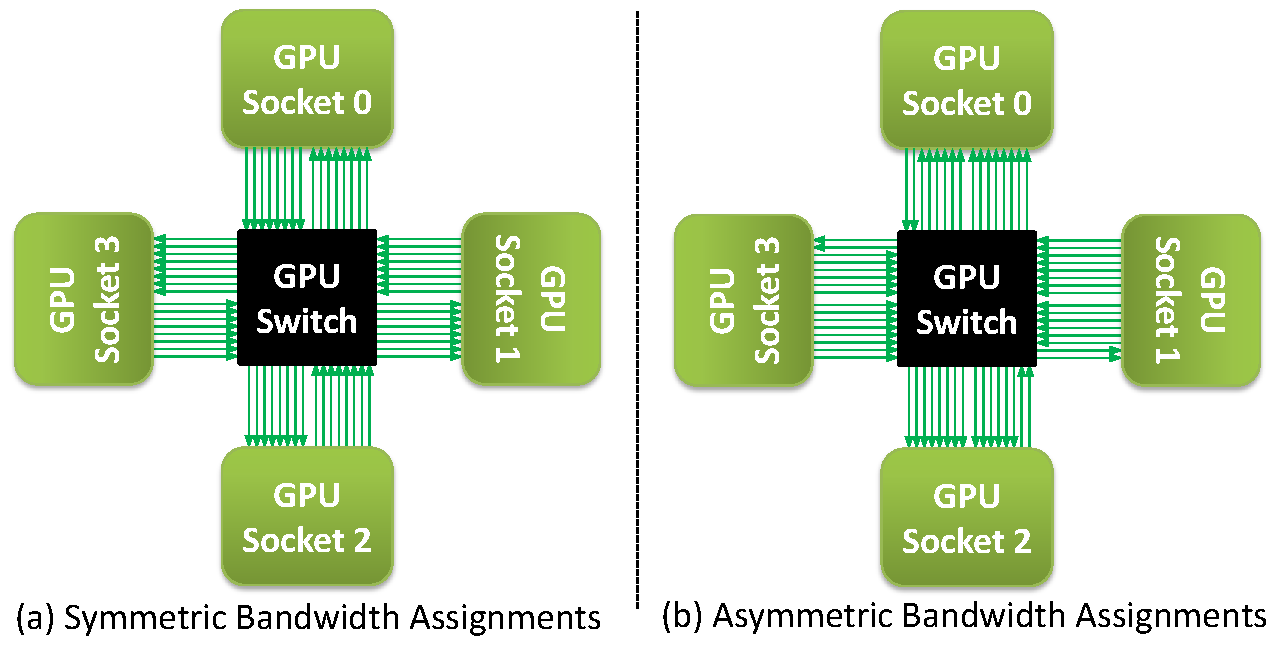
\includegraphics[width=1.0\columnwidth]{figures/tms_links.pdf}
    \caption{Multi-socket GPU systems with symmetric and assymeteric link
    bandwidth assignments.}
    \label{fig:symmetric_assymetric}
\end{figure}

In many other workloads we also observe inter-socket traffic patterns that
would be better of with an asymmetric link bandwidth allocation. A common
scenario is writing to the same memory section by all CTAs at the end of a
kernel (i.e. parallel reductions, data gathering). For CTAs running on one of the
sockets, GPU0 for example, these memory instructions are local and do not
produce any traffic on the inter-socket interconnections. While CTAs dispatched
to other GPUs issue remote memory writes, saturating their egress links while
ingress links remain underutilized. Such a communication pattern utilizes only
50\% of available bandwidth. In such case, increasing the number of ingress lanes for GPU0
(by turning around direction of egress lanes), and switching the direction of
ingress lanes for all other GPUs, could substantially improve the performance
by effectively providing 2x larger bandwidth on the same wires. 

Motivated by these findings, we propose to dynamically control multi-socket
link bandwidth assignments in each direction on a per-GPU basis resulting in
dynamically asymmetric link capacity assignments, as shown in
Figure~\ref{fig:symmetric_assymetric}(b). Such dynamic and asymmetric link
capacity distribution is expected to yield higher wire utilization and
essentially higher effective bandwidth and performance for a given set of I/O
resources. This mechanism is somewhat similar to DRAM interface for example,
where the same set of wires is used for both read and write directions
interchangeably, and link direction is reversed based on a dynamic state of the
system~\cite{jedecDDR3}. 

For basic link configuration we assume and model point-to-point links with
multiple lanes each, similarly to NVLink sub-links~\cite{pascal-tesla-wp}. In
such link, 8 lanes with 8GB/s capacity per lane yield an aggregate bandwidth of
64GB/s in each direction. We propose to replace uni-directional lanes with
bi-directional lanes, and then we develop and apply an adaptive asymmetric link
bandwidth allocation mechanism that works as following. For each link in the
system, at kernel launch we start with symmetric link bandwidth assignments
with 8 lanes per direction. Then, we periodically sample the saturation status
of each link. If the lanes in one direction are not saturated, while the lanes
in the opposite direction are 99\% saturated, we reverse the direction of one
of the unsaturated lanes. Repeating the previous step and sampling the lanes
status, we stop either when equilibrium is reached, or alternatively all the
lanes but one have been reversed (we always keep a minimum bandwidth of 8GB/s
in each direction).  



\begin{figure}[t]
    \centering
    
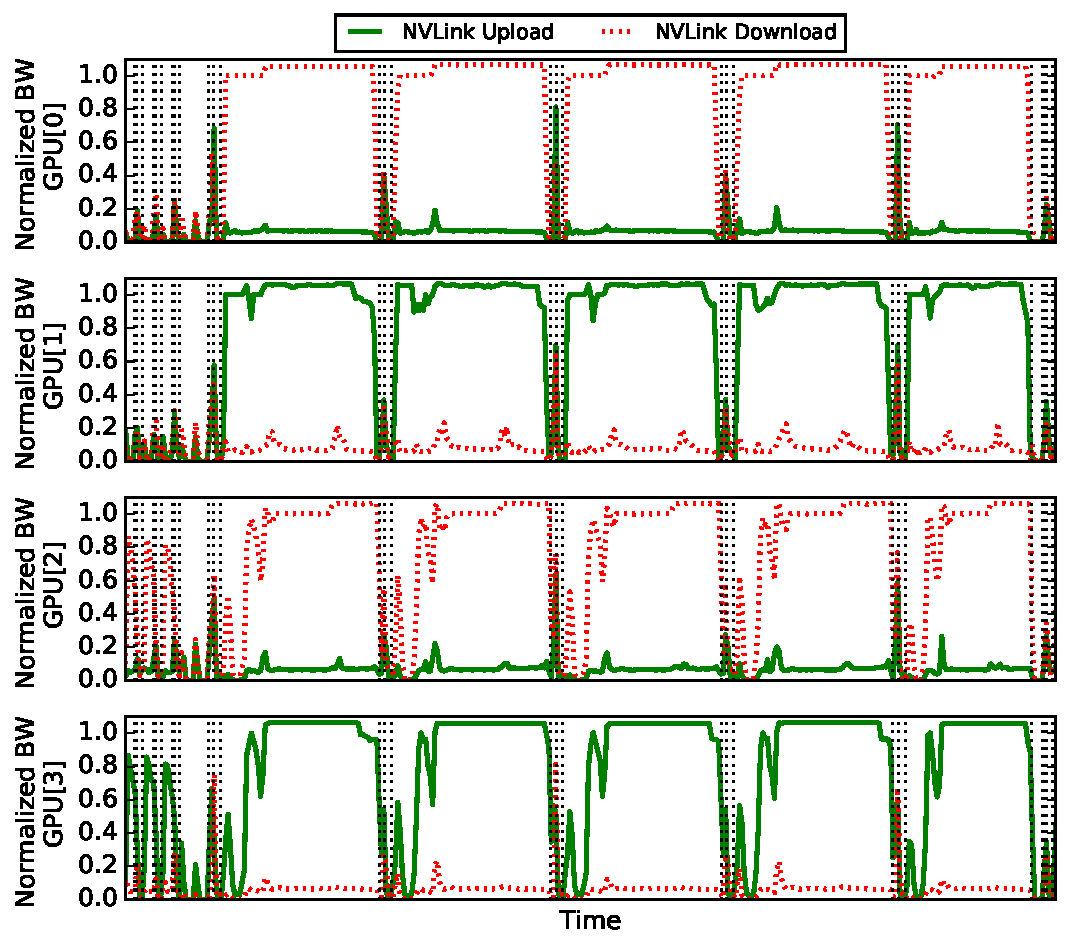
\includegraphics[width=1.0\columnwidth]{figures/bw_profile_HPGMG_UVM_base.pdf}
    \caption{Normalized NVLink bandwidth profile for \texttt{HPC-HPGMG-UVM} 
showing example of asymmetric 
    link utilization between GPUs and within a GPU depending on kernel and 
application phasing.}
    \label{fig:link-motivation}
\end{figure}

\begin{figure*}[tp]
    \centering
    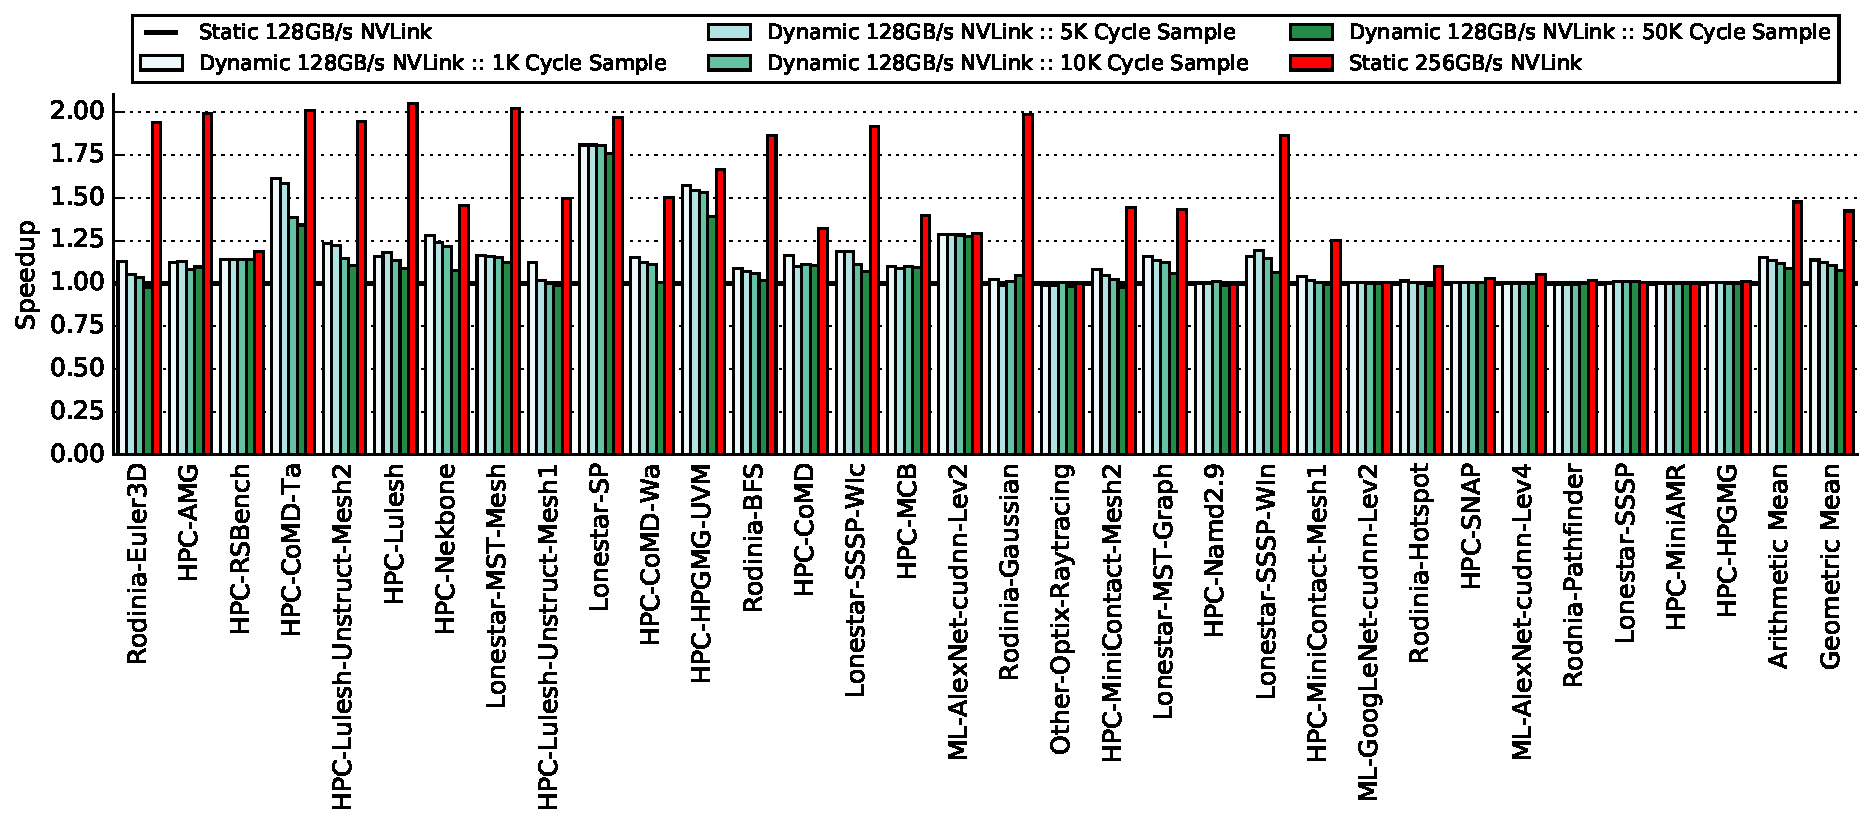
\includegraphics[width=1.0\textwidth]{figures/plot_nvlink_sample_time.pdf}
    \caption{Relative speedup of the dynamic NVlink adaptivity with respect to
	the baseline architecture by varying sample time and assuming switch 
time of
	100 cycles. In red, relative speedup achievable by doubling the 
bandwidth.}
    \label{fig:sampletime}
\end{figure*}

\subsection{Link Results and Discussion} 

There are two important parameters that characterize the proposed mechanism (i)
\texttt{SampleTime}: the frequency at which the scheme samples for a possible
reconfiguration and (ii) \texttt{SwitchTime}: the cost of switching the
direction of a lane. Switching period is comprised of the time it takes to
drain all the pending packets in a given direction, and the time it takes to
physically reconfigure the lane to start transmitting in the opposite
direction.  Figure~\ref{fig:sampletime} shows the performance improvement, with
respect to our baseline architecture by exploring different values of the
\texttt{SampleTime} indicated by greenn bars and assuming a \texttt{SwitchTime}
of 100 cycles which is a typical switching time for a high-speed serial
link~\cite{XXX}. The red bars in Figure~\ref{fig:sampletime} provide an
upper-bound performance speedups when doubling the available interconnect
bandwidth to 256GB/s. For the benchmarks on the right side, where the baseline
4 GPU multi-socket system performs close to 4$\times$ larger single GPU,
increasing the inter-socket bandwidth does not improve performance
significantly.  Contiguous CTA scheduling and first-touch memory placement
preserves good data locality in these cases, so that both ingress and egress
links are underutilized. On the left side, we can see that for some
applications, 2$\times$ NVLink bandwidth translates to 2$\times$ speedup, while
dynamic lane switching achieves up to 80\% performance improvement
(\texttt{Lonestar-SP}).  We can see that doublng the interconnect bandwidth
achieves 50\% speedup on average, while our proposed dynamic mechanism achieves
15\% speedup on average (with 5K sample period). We show that the sampling frequency
plays a critical role, long sample times do not capture application dynamics
resulting in smaller perfromance improvements. Our findings indicate that 5K
cycles can be a good sampling period, and sample times below that achieve
deminishing results.

In addition we observe that for benchmarks like \texttt{Rodinia-Euler-3D}, \texttt{HPC-AMG}, and 
\texttt{HPC-Lulesh}, doubling the NVLink bandwidth provides 2$\times$ 
speedup, while our proposed dynamic link assignment mechanism is not 
able to significantly improve performance. Those are the workloads 
that saturate both link directions, so there is no opportunity to 
provide additional bandwidth by turning links around. For the rest of 
the applications on the left side, performance improvement is directly 
proportional to the actual link utilization of unsaturated lanes. For 
example, consider a case where a GPU fully saturates its egress links 
and incoming traffic achieves only 75\% of ingress bandwidth (using 6 
out of 8 lanes). Then, adaptive policy is able to increase the outgoing 
bandwidth for a maximal 25\% by turning around those 2 unused ingress 
lanes. If such a traffic communication pattern is sustained throughout 
50\% of the total execution time, the maximal performance improvement 
that our dynamic link assignment can achieve is 12.5\%.

Another important design parameter is switching period needed to turn around a
single lane direction. Our results point that higher \texttt{SwitchTime}
values, like 200 and 500 cycles, degrade the average performance by less than
2\% compared to 100 cycle switching period. We observe the maximum slowdown of
25\% in case of \texttt{HPC-CoMD-Ta} and \texttt{HPC-CoMD-Wa} when switch time
reaches 500 cycles. At the same time, faster lane switch (10 cycles) does not
improve the performance compared to 100 cycles. Thus from now, we define our
adaptive link assignment policy which samples saturation status on every 5K
cycles and eventually turn link direction with 100 cycles penalty.

Our results demonstrate that the proposed dynamic and asymmetric link
bandwidth allocation can be very attractive in multi-socket GPU realm, where
inter-socket interconnect bandwidth is limited by the number of on-PCB wires
and the non-scaling die-edge dimensions for breaking out of the chip boundaries
onto the package. We can see that our mechanisms improved application
performance by 14\% on average and with some applications seeing up to 81\%
performance speedups (i.e. Lonestar), however they do not come without a cost.
The main drawback of this solution is that both types of interface circuitry
and logic need to be implemented for each lane in GPU and Switch interfaces, moreover
even though total switch bandwidth stays always constant, and cannot exceed the 
maximal bandwidth of per-link lanes multiplied by the number of links, 
the internal switch fabric might need to be redesigned to support
asymmetric traffic patterns. We believe our proposed mechanism may motivate
future research in the domain of asymmetric switch architecture, however we
keep it out of the scope of this paper.

 

% DO NOT REMOVE, we can use this to compute POWER later 
%from http://teams.nvidia.com/sites/Corporate/ntech/SiteAssets/downloads/2014/NTECH2014_SlideDecks20(presented)/7.1_Osborn.pptx 
%Power: 8 lanes (TX + RX) at 25GT/s ~= 1.5W 
%Area: 8 Lane PHY (8 TX + 8 RX + PLL) ~= 3.3mm^2 %Physical Data: .5pJ/b transferred



